%!TEX root = ../thesis.tex

\chapter*{Quick overview of useful LateX Commands}



\section{Sidenotes}\label{sec:sidenotes}
One of the most prominent and distinctive features of this style is the
extensive use of sidenotes.  There is a wide margin to provide ample room
for sidenotes and small figures.  Any \doccmd{footnote}s will automatically
be converted to sidenotes.\footnote{This is a sidenote that was entered
using the \texttt{\textbackslash footnote} command.}  If you'd like to place ancillary
information in the margin without the sidenote mark (the superscript
number), you can use the \doccmd{marginnote} command.\marginnote{This is a
margin note.  Notice that there isn't a number preceding the note, and
there is no number in the main text where this note was written.}

The specification of the \doccmddef{sidenote} command is:
\begin{docspec}
\doccmd{sidenote}[\docopt{number}][\docopt{offset}]\{\docarg{Sidenote text.}\}
\end{docspec}

Both the \docopt{number} and \docopt{offset} arguments are optional.  If you
provide a \docopt{number} argument, then that number will be used as the
sidenote number.  It will change of the number of the current sidenote only and
will not affect the numbering sequence of subsequent sidenotes.

Sometimes a sidenote may run over the top of other text or graphics in the
margin space.  If this happens, you can adjust the vertical position of the
sidenote by providing a dimension in the \docopt{offset} argument.  Some
examples of valid dimensions are:
\begin{docspec}
  \ttfamily 1.0in \qquad 2.54cm \qquad 254mm \qquad 6\Verb|\baselineskip|
\end{docspec}
If the dimension is positive it will push the sidenote down the page; if the
dimension is negative, it will move the sidenote up the page.

While both the \docopt{number} and \docopt{offset} arguments are optional, they
must be provided in order.  To adjust the vertical position of the sidenote
while leaving the sidenote number alone, use the following syntax:
\begin{docspec}
  \doccmd{sidenote}[][\docopt{offset}]\{\docarg{Sidenote text.}\}
\end{docspec}
The empty brackets tell the \Verb|\sidenote| command to use the default
sidenote number.

If you \emph{only} want to change the sidenote number, however, you may
completely omit the \docopt{offset} argument:
\begin{docspec}
  \doccmd{sidenote}[\docopt{number}]\{\docarg{Sidenote text.}\}
\end{docspec}

The \doccmddef{marginnote} command has a similar \docarg{offset} argument:
\begin{docspec}
  \doccmd{marginnote}[\docopt{offset}]\{\docarg{Margin note text.}\}
\end{docspec}


\section{Citations}

To cite previous work or various other sources (websites, APIs, etc.), you can use the command:
\begin{docspec}
  \doccmd{cite}\{\docarg{citation entry}\}
\end{docspec}
The citation entry must be part of your .bib file (by default \textit{bibliography.tex} in the \textit{backmatter} folder). To cite multiple source at once, you can add a coma between them:
\begin{docspec}
  \doccmd{cite}\{\docarg{entry1, entry2, entry3, ...}\}
\end{docspec}
Here is an example~\cite{Tufte2006} and here is another~\cite{Tufte1990, Tufte1997, Tufte2001}.




\section{Tables}

You can simply create tables, as the one shown below.

\begin{table}[h]
  \footnotesize%
  \begin{center}
    \begin{tabular}{lccl}
      \toprule
      \LaTeX{} size & Font size & Leading & Used for \\
      \midrule
      \verb+\tiny+         &  5 &  6 & sidenote numbers \\
      \verb+\scriptsize+   &  7 &  8 & \na \\
      \verb+\footnotesize+ &  8 & 10 & sidenotes, captions \\
      \verb+\small+        &  9 & 12 & quote, quotation, and verse environments \\
      \verb+\normalsize+   & 10 & 14 & body text \\
      \verb+\large+        & 11 & 15 & \textsc{b}-heads \\
      \verb+\Large+        & 12 & 16 & \textsc{a}-heads, \textsc{toc} entries, author, date \\
      \verb+\LARGE+        & 14 & 18 & handout title \\
      \verb+\huge+         & 20 & 30 & chapter heads \\
      \verb+\Huge+         & 24 & 36 & part titles \\
      \bottomrule
    \end{tabular}
  \end{center}
  \caption{This is the caption of a table. This table lists all the various font sizes available.}
  \label{tab:font-sizes}
\end{table}

To refer to a table, you can use the \verb+\ref{<table's label>}+ command like this Table~\ref{tab:font-sizes}.



\section{Figures}
Images and graphics play an integral role in Tufte's work.
In addition to the standard \docenvdef{figure} and \docenvdef{tabular} environments,
this style provides special figure and table environments for full-width
floats.

Full page--width figures and tables may be placed in \docenvdef{figure*} or
\docenvdef{table*} environments.  To place figures or tables in the margin,
use the \docenvdef{marginfigure} or \docenvdef{margintable} environments as follows
(see figure~\ref{fig:marginfig}):

\begin{marginfigure}%
  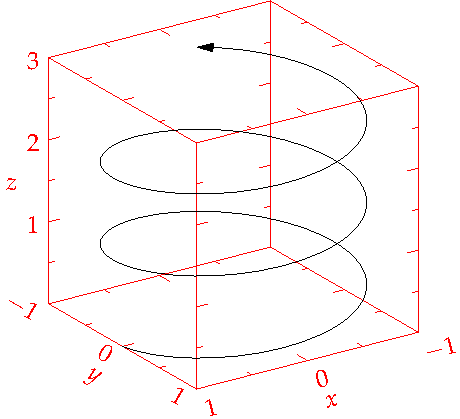
\includegraphics[width=\linewidth]{images/helix}
  \caption{This is a margin figure.  The helix is defined by 
    $x = \cos(2\pi z)$, $y = \sin(2\pi z)$, and $z = [0, 2.7]$.  The figure was
    drawn using Asymptote (\protect\url{http://asymptote.sf.net/}).}
  \label{fig:marginfig}
\end{marginfigure}

\begin{docspec}
\textbackslash begin\{marginfigure\}\\
  \qquad\textbackslash includegraphics\{helix\}\\
  \qquad\textbackslash caption\{This is a margin figure.\}\\
  \qquad\textbackslash label\{fig:marginfig\}\\
\textbackslash end\{marginfigure\}\\
\end{docspec}

The \docenv{marginfigure} and \docenv{margintable} environments accept an optional parameter \docopt{offset} that adjusts the vertical position of the figure or table.  See the ``\nameref{sec:sidenotes}'' section above for examples.  The specifications are:
\begin{docspec}
  \textbackslash{begin\{marginfigure\}[\docopt{offset}]}\\
  \qquad\ldots\\
  \textbackslash{end\{marginfigure\}}\\
  \mbox{}\\
  \textbackslash{begin\{margintable\}[\docopt{offset}]}\\
  \qquad\ldots\\
  \textbackslash{end\{margintable\}}\\
\end{docspec}

Figure~\ref{fig:fullfig} is an example of the \docenv{figure*}
environment and figure~\ref{fig:textfig} is an example of the normal
\docenv{figure} environment.

\begin{figure*}[h]
  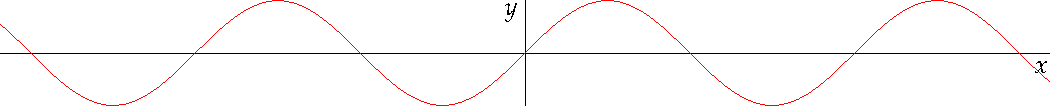
\includegraphics[width=\linewidth]{images/sine.pdf}%
  \caption{This graph shows $y = \sin x$ from about $x = [-10, 10]$.
  \emph{Notice that this figure takes up the full page width.}}%
  \label{fig:fullfig}%
\end{figure*}

\begin{figure}
  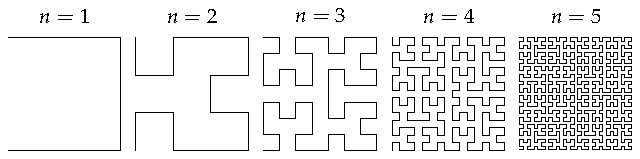
\includegraphics{images/hilbertcurves.pdf}
%  \checkparity This is an \pageparity\ page.%
  \caption{Hilbert curves of various degrees $n$. \emph{Notice that this figure only takes up the main textblock width.}}
  \label{fig:textfig}
  %\zsavepos{pos:textfig}
\end{figure}

As with sidenotes and marginnotes, a caption may sometimes require vertical
adjustment. The \doccmddef{caption} command now takes a second optional
argument that enables you to do this by providing a dimension \docopt{offset}.
You may specify the caption in any one of the following forms:
\begin{docspec}
  \doccmd{caption}\{\docarg{long caption}\}\\
  \doccmd{caption}[\docarg{short caption}]\{\docarg{long caption}\}\\
  \doccmd{caption}[][\docopt{offset}]\{\docarg{long caption}\}\\
  \doccmd{caption}[\docarg{short caption}][\docopt{offset}]%
                  \{\docarg{long caption}\}
\end{docspec}
A positive \docopt{offset} will push the caption down the page. The short
caption, if provided, is what appears in the list of figures/tables, otherwise
the ``long'' caption appears there. Note that although the arguments
\docopt{short caption} and \docopt{offset} are both optional, they must be
provided in order. Thus, to specify an \docopt{offset} without specifying a
\docopt{short caption}, you must include the first set of empty brackets
\Verb|[]|, which tell \doccmd{caption} to use the default ``long'' caption. As
an example, the caption to figure~\ref{fig:textfig} above was given in the form
\begin{docspec}
  \doccmd{caption}[Hilbert curves...][5em]\{Hilbert curves...\}
\end{docspec}


Pictures can also be placed next to each other:
\begin{figure*}
\resizebox{\textwidth}{!}{% \hspace*{-0.2em}
	\subfloat[]{%
	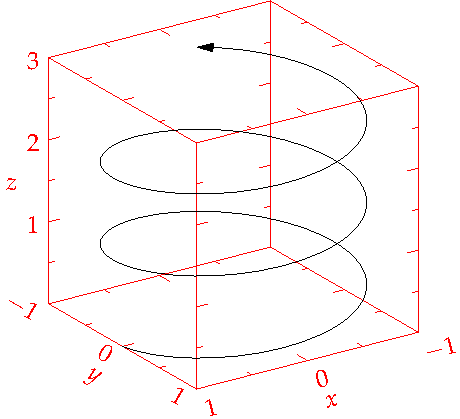
\includegraphics[height=3cm]{images/helix.pdf}%
	}\hspace{0.05em}
	\subfloat[]{%
	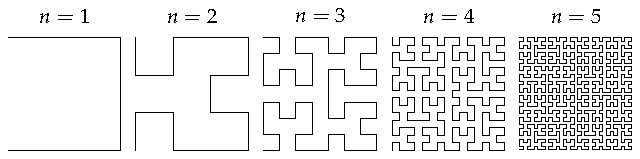
\includegraphics[height=3cm]{images/hilbertcurves.pdf}%
	}
}
\caption{PIctures are aligned on the same line, and automatically annotated with letters.}
\label{fig:ushaped}
\end{figure*}

\section{Full-width text blocks}

In addition to the new float types, there is a \docenvdef{fullwidth}
environment that stretches across the main text block and the sidenotes
area.

\begin{Verbatim}
\begin{fullwidth}
Lorem ipsum dolor sit amet...
\end{fullwidth}
\end{Verbatim}

\begin{fullwidth}
\small\itshape\lipsum[1]
\end{fullwidth}


\section{Sections and subsections}

This is a section. Sections and subsections appear in the Table of Contents (ToC), so rely heavily on them to structure your text and your argumentation.

\subsection{This is a first subsection...}

\subsection{... and here is a second}
